\section{Slabs: split targets and the corrected criterion}\label{sec:slab}
Suppose the target splits along the third coordinate with period $k$: $\Lambda'=\Lambda'_2\oplus k\Z e_3$, with $\Lambda'_2$ a rank-two lattice in the $(x_1,x_2)$-plane. (The symbol $k$ is the period here, not the dimension.) For $k=1$ the coordinate is \emph{free} ($e_3\in\Lambda'$). Write $Q=(Q',q_3)$, $J=\lfloor q_3/k\rfloor$, $U=U(\Lambda'_2,Q')$ and $U^0=U^0(\Lambda'_2,Q')$ (planar, origin excluded, resp.\ allowed). The three-dimensional union is a stack of planar unions with a single exceptional layer.

\subsection{The union of a split target}
\begin{theorem}[slab structure]\label{thm:slab-i}
For $J\ge1$, $U(\Lambda',Q)=\bigl[U\times[0,k]\bigr]\cup\bigl[U^0\times[k,kJ]\bigr]$; for $J=0$, $U(\Lambda',Q)=U\times\{0\}$.
\end{theorem}
\prov{CW-0511}{P5-S4}{PROVED}{FULL}
\begin{proof}
A nonzero vector $(a,t)$ of $\Lambda'$ with $a\ne0\ne t$ has $(a,0)\in\Lambda'$ conformally below it, so it is not Graver; $(a,0)$ is Graver in $\Lambda'$ iff $a$ is Graver in $\Lambda'_2$; $(0,t)$ is Graver iff $|t|=k$. So $\Gr(\Lambda')=\{(g,0):g\in\Gr(\Lambda'_2)\}\cup\{\pm ke_3\}$ and every cell of $\Lambda'$ is $c_2\times\{z\}$ or $c_2\times[z,z+k]$ with $c_2$ a planar cell (generators in $\Gr(\Lambda'_2)$), $z\in k\Z$, $z\ge0$ (and $z+k\le q_3$ in the second case). The corner $(v,z)$ is zero iff $v=0$ and $z=0$. For $z=0$ the planar factor must avoid the corner $0$: $c_2$ is a cell of $U$; for $z\ge k$ the origin is allowed: $c_2$ is a cell of $U^0$. In the second form the corners with third coordinate $z+k\ge k$ impose nothing more. Taking the union over $z$: heights in $[0,k]$ are covered by cells with $z=0$ (giving $U$ at heights $<k$) and heights in $[k,kJ]$ by cells with $z\ge k$ (giving $U^0$); at height exactly $k$ both occur and $U\subseteq U^0$. For $J=0$ only $z=0$ and no $\pm ke_3$ exist. \qedhere
\end{proof}
\begin{corollary}[free coordinate: slab lemma]\label{cor:slab-lemma}
If $e_3\in\Lambda'$ ($k=1$) and $q_3\ge1$ then for $0<c<1$: $(x',c)\in U(\Lambda',Q)\iff x'\in U(\Lambda'_2,Q')$; and for $c\in[1,q_3]$ the slice is $U^0$. If a point $p\in U(\Lambda,Q)$ has $0<p_3<1$ and its planar part lies outside $U(\Lambda'_2,Q')$, then $U(\Lambda,Q)\not\subseteq U(\Lambda',Q)$ (slab obstruction).
\end{corollary}
\prov{CW-0492}{P4-S1}{PROVED}{FULL}
\prov{CW-0494}{P4-S2}{PROVED}{ADAPTED}
\begin{proof}
\Cref{thm:slab-i} with $k=1$. \qedhere
\end{proof}
The slab lemma shows that a free-coordinate obstruction is inherited from the planar target: a planar gap times a thin slab. It is not a new three-dimensional coupling.

\subsection{The corrected containment criterion}\label{sec:slab-ii}
\begin{theorem}[containment criterion, corrected form]\label{thm:slab-ii}
Let $\Lambda\subseteq\Lambda'=\Lambda'_2\oplus k\Z e_3$ and let $c$ be a cell of $U(\Lambda,Q)$. Then
\[
c\subseteq U(\Lambda',Q)\iff\Bigl[\ \min_{x\in c}x_3\ge k\ \Bigr]\ \text{ or }\ \Bigl[\ \mathrm{proj}_{12}\bigl(c\cap\{x_3\le k\}\bigr)\subseteq U(\Lambda'_2,Q')\ \Bigr].
\]
Equivalently: $c\subseteq U(\Lambda',Q)$ iff $\mathrm{proj}_{12}(c\cap\{x_3<k\})\subseteq U$.
\end{theorem}
\prov{CW-0511}{P5-S4(ii)'}{PROVED}{FULL}
\begin{proof}
The corners of $c$ lie in $\Lambda\subseteq\Lambda'$, so their third coordinates lie in $k\Z\cap[0,q_3]$, and $c\subseteq\{0\le x_3\le kJ\}$. By \cref{thm:slab-i} the slice of $U(\Lambda',Q)$ at height $z<k$ is $U$ and at height $z\in[k,kJ]$ is $U^0$ (for $J=0$ the cell lies in $\{x_3=0\}$ and the slice is $U$). Hence $c\subseteq U(\Lambda',Q)$ iff (a) $\mathrm{proj}_{12}(c\cap\{x_3<k\})\subseteq U$ and (b) $\mathrm{proj}_{12}(c\cap\{k\le x_3\le kJ\})\subseteq U^0$.

\emph{Claim: (b) always holds, indeed $\mathrm{proj}_{12}(c)\subseteq U^0$.} The projection of $c=\Pil(u;g_1,\dots,g_j)$ is the zonogon $\mathrm{proj}(u)+\sum[0,1]\mathrm{proj}(g_l)$ where $\mathrm{proj}(g_l)\in\Lambda'_2$ (the projection maps $\Lambda'$ into $\Lambda'_2$); its corners are projections of corners of $c$, hence lie in $\Lambda'_2\cap Q'$ (the origin allowed). Decompose each $\mathrm{proj}(g_l)$ by \cref{lem:L1} into Graver vectors of $\Lambda'_2$ conformally below it and tile the zonogon by \cref{lem:T0}. As in the proof of \cref{prop:Z} (Z.1), every tile vertex is the sum of the base and partial sums of the pieces; its coordinates lie between coordinates of corners of the projected cell, hence in $[0,Q']$, and it lies in $\Lambda'_2$. With the origin allowed, every tile is a cell of $U^0$, so $\mathrm{proj}(c)\subseteq U^0$.

Therefore $c\subseteq U(\Lambda',Q)$ iff (a). If $c\cap\{x_3<k\}=\emptyset$ (that is $\min x_3\ge k$) (a) is vacuous. Otherwise $c\cap\{x_3<k\}$ is a nonempty convex subset of the convex set $c$ whose closure is $c\cap\{x_3\le k\}$ (move from any point of $c\cap\{x_3\le k\}$ towards a point with $x_3<k$); since $U$ is closed and the projection is continuous, (a) is equivalent to $\mathrm{proj}(c\cap\{x_3\le k\})\subseteq U$. \qedhere
\end{proof}
\begin{remark}[the erratum]\label{rem:E1}
The first release of this criterion (v005, P5-S4(ii)) stated the condition $\mathrm{proj}_{12}(c\cap\{x_3\le k\})\subseteq U$ \emph{without} the alternative $\min x_3\ge k$. That closed-height form is false, and it is \emph{not} stated as valid here. Counterexample (erratum E1, ER-22, reproduced independently here): $\Lambda=2\Z^2\oplus2\Z$, $\Lambda'=\Z^2\oplus2\Z$ (period $k=2$), $Q=(2,2,2)$, $c=[0,2]^2\times\{2\}=\Pil((0,0,2);(2,0,0),(0,2,0))$. Then $c$ is a source cell and $c\subseteq U(\Lambda',Q)$ (for instance $(\tfrac12,\tfrac12,2)\in U(\Lambda',Q)$ because at height $2=k$ the target already contains the vertex $(0,0,2)\ne0$, so its slice there is $U^0$, not $U$); but the closed-height criterion would reject $c$ because $(\tfrac12,\tfrac12)\notin U(\Z^2,(2,2))$. All earlier consequences of the \emph{hard-cell} comparisons were unaffected: a hard cell has $\min x_3=0<k$, where the closed form is correct.
\end{remark}

\begin{figure}[tbp]\centering
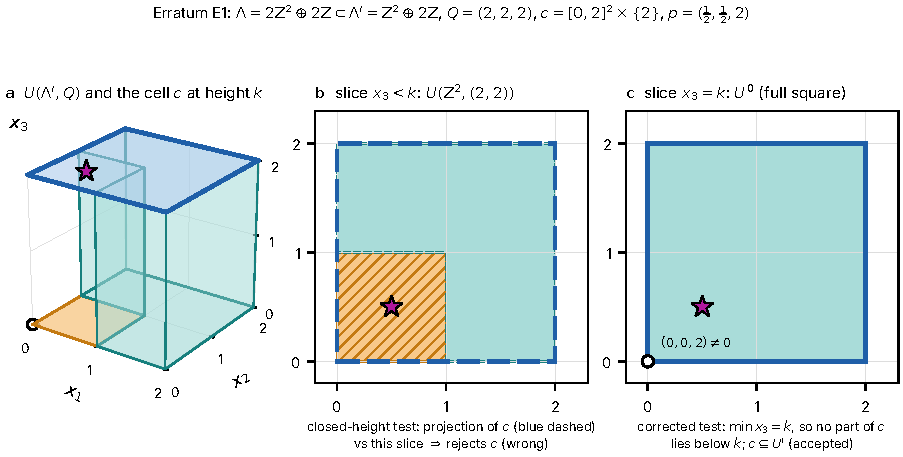
\includegraphics[width=0.98\textwidth]{fig13_strict_slab}
\caption{Why the strict-slab correction matters (\cref{thm:slab-ii}, \cref{rem:E1}; $\Lambda=2\Z^2\oplus2\Z\subset\Lambda'=\Z^2\oplus2\Z$, $k=2$, $Q=(2,2,2)$; \emph{exact computation}). The cell $c=[0,2]^2\times\{2\}$ lies at height $x_3=k$. (a)~$U(\Lambda',Q)$ and $c$. (b)~The slice $x_3<k$ is the origin-excluded $U(\Z^2,(2,2))$, which does not contain $(\frac12,\frac12)$. (c)~The slice $x_3=k$ is the origin-allowed full square $U^0$. The point $p=(\frac12,\frac12,2)$ lies in $U(\Lambda',Q)$ (and all $121$ grid points of $c$ do), so $c\subseteq U(\Lambda',Q)$ and the corrected criterion (strict height $x_3<k$; here $c\cap\{x_3<k\}=\emptyset$) accepts $c$. The closed-height form of the first release would require $\mathrm{proj}_{12}(c)\subseteq U(\Z^2,(2,2))$, which fails at $(\frac12,\frac12)$, and would wrongly reject $c$.}\label{fig:strict}
\end{figure}
\subsection{The free-coordinate case}
\begin{corollary}[complete slab criterion]\label{cor:S3}
Let $e_3\in\Lambda'$ ($k=1$), $q_3\ge1$ and $\Lambda\subseteq\Lambda'$. Then $U(\Lambda,Q)\subseteq U(\Lambda',Q)$ iff there is no point $p\in U(\Lambda,Q)$ with $p_3<1$ whose planar part lies outside $U(\Lambda'_2,Q')$.
\end{corollary}
\prov{CW-0498}{P4-S3}{PROVED}{ADAPTED}
\begin{proof}
\Cref{thm:slab-ii} with $k=1$, applied to every cell: $c\subseteq U'$ iff $\mathrm{proj}(c\cap\{x_3<1\})\subseteq U$. \qedhere
\end{proof}
In particular, for free-coordinate targets every failure is a slab obstruction (the ``S1 failures'' of the intermediate releases do not exist), and the failures of this class are exactly the planar target gaps seen through the layer $0<x_3<1$. The slab criterion is drawn in \cref{fig:slab}.
\begin{figure}[tbp]\centering
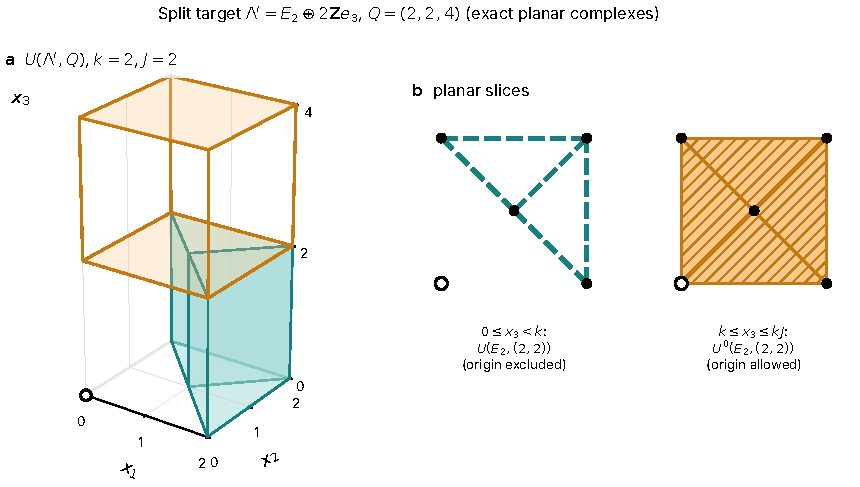
\includegraphics[width=0.98\textwidth]{fig12_slab_structure}
\caption{Geometry of a split target (\cref{thm:slab-i}; $\Lambda'=E_2\oplus2\Z e_3$, $Q=(2,2,4)$, $k=2$, $J=2$; planar complexes \emph{exact}, vertical stacking \emph{schematic}). (a)~The union $U(\Lambda',Q)$: below height $k$ the slice is the origin-excluded planar union $U=U(E_2,(2,2))$ (blue; one-dimensional here, $5$ edges and no square), from height $k$ upward it is the origin-allowed union $U^0$ (orange; the filled square $[0,2]^2$ and $8$ edges). (b)~The two planar slices. A source cell is contained iff its part below height $k$ projects into $U$. The figure shows a realised union, not an abstract complex.}\label{fig:slab}
\end{figure}
